\chapter{Reinforcement Learning}



\section{What is Reinforcement Learning}


\subsection{Constituents of a RL System}

\begin{itemize}
    \item Environment:
          Has an internal state $\bar{S_t}$ (true state), Takes an action $A_t$ and returns Observation $O_t$.
    \item Reward Signal:
          Takes the Observation $O_t$ to returns a reward $R_t$ not mutable by the agent.
    \item Agent (Learning algorithm):
          Has a State $S_t$, Value Function, Policy, Model (optionally).
\end{itemize}

Return is the sum of rewards over all steps: $G_t = G_{t − 1} + R_t$.

The goal is to maximize the following:
\begin{equation}
    q(s, a) = E[G_t ∣ S_t = s, A_t = a] = E[R_{t_1} + R_{t_2} + \dots ∣ S_t = s, A_t = a]
\end{equation}


\subsection{Terms relation to the state}

\subsubsection{State of the Environment}

History is defined to be the set of all actions and observations with which we can recreate the current state: $ H_t = A_0 O_0 A_1 O_1 \dots A_n O_n $

Fully Observable State are defined to have: $S_t = O_t$, that is the current observation represents the entire state of the game.

For Partially observable environments, we can represent the state using a Recurrent Neural Network with Memory to store some features of the history.

The state may be Markovian only to the environment and not to the agent, if there are additional unknows for the agent.

\begin{definition}[Markov Decision Process]{def:mdp}
    A decision process is Markovian if: $p(r, s ∣ S_t, A_t) = p(r, s ∣ H_t, A_t)$, i.e. the future is independent of the part given the present ($H_t \rightarrow S_t \rightarrow H_t+1$).
\end{definition}

One of the reasons why an environment is not Markov is because it's non-stationary (and we don't want to or can't model how the environment evolved)

\subsubsection{State of the Agent}

\begin{theorem}[Bellman Equations]{thm:bellman-equations}
    \begin{eqnarray}
        v_\pi &=& E[E_t + 1 + \gamma G_t + 1 ∣ S_t = s, A_t \sim \pi(s)] \\
        &=& E[E_t + 1 + \gamma v_\pi(S_t+1) ∣ S_t=s, A_t \sim \pi(s)]
    \end{eqnarray}
\end{theorem}

The same holds true for the optimal value function (this equation is independent of the policy):
\begin{equation}
    v_∗ = max_a[E_t + 1 + \gamma v_∗ G_t + 1 | S_t = s, A_t = a]
\end{equation}
Agents often approximate the value function.

\subsubsection{Model of the Environment}

Transition probabilities:
\begin{equation}
    P(s, a, s^\prime) = P(S_t + 1 = s^\prime ∣ S_t = s, A_t = a)
\end{equation}

Immediate reward:
\begin{equation}
    R(s, a) = E[R_t + 1 ∣ S_t = s, A_t = a]
\end{equation}



\section{Exploration and Exploitation}

\emph{In this section we are taking the example of the Multi-Arm Bandit, the major assumption is that the length of the episode is 1, our actions do not affect our state.}

The true value of the action is: $q(a) = E[R_t | A_t = a]$.
\begin{note}[Q-Value Update]{note:q-value-update}
    We have an approximation on the value, we can update as follows:
    \begin{eqnarray}
        Q_t(a) &=& \frac{\sum_{n=1}^{t} R_n I(A_n = a)}{\sum_{n=1}^{t} I(A_n = a)} \\
        Q_t(A_t) &=& Q_{t-1}(A_t) + \alpha_f(R_f - Q_{t-1}(A_t))
    \end{eqnarray}
\end{note}


\subsection{Lower Bound on Regret}

Regret is the value by which we got the rewards wrong:
\begin{equation}
    G = \sum_t (v_* - q(A_t)) = \sum_a N(a) (v_* - q(a))
\end{equation}
We want to minimize the regret over the training-cum-test period (we can forever keep learning).

If we use methods like $\epsilon$-Greedy (explore some times and exploit other times), our regret growth is still linear in the length of time, which is only constant factor better from learning nothing.

We can prove the lower bound that Asymptotic total regret is at least Logrithmic in the number of steps. This is formally described by the gap $\Delta_a = (v_* - q(a))$.
\begin{equation}
    \lim_{t \rightarrow \infty} L_t \geq log(t) \sum_{a \vert \Delta_a > 0} \frac{\Delta_a}{KL(p(r \vert a) \Vert p(r \vert a_*))}
\end{equation}
The regret is still unbounded, but it's lower-bounded by logrithm in $t$.


\subsection{Upper Confidence Bound}

\textbf{Hoeffding's Inequality} is a concentration bound result. Given independent and identically distributed random variables $X_1, X_2, \dots X_n$, let $\bar{X} = \frac{1}{n} \sum_{i=1}^{n} X_i$ be the sample mean. Then:
\begin{equation}
    p((\mathbb{E}[X] - \bar{X}) < u) = e^{-2nu^2}
\end{equation}

If we assume that are rewards are in the range [0, 1), then we can derive the relation for the upper confidence bound for probability p (the maximum range we can be sure the rewards are in with probability atleast p):
\begin{eqnarray*}
    p(q(a) \geq Q_t(a) + U_t(a)) &\leq& e^{-2N_t(a)U_t(a)^2} \\
    \implies U_t(a) &=& \sqrt{\frac{-\log(p)}{2N_t(a)}}
\end{eqnarray*}
The root over the number of observations is due to the assumptions that the variables are IID, using central limit theorem our confidences are gaussians, the standard deviation for it is proportional to root of n.

We want to set p increasing proportionally to time. So we can replace p with n.

\begin{algo}[UCB algorithm]{algo:ucb-algo}
    \begin{equation}
        a_t = argmax_{a \in \mathcal{A}} Q_t(a) + c\sqrt{\frac{log t}{N_t(a)}}
    \end{equation}
    c is a hyperparameter which represent learning rate of some sort (usually 1 to 2).

    Setting $c = \sqrt{2}$, the Logrithmic lower bound (upto constant) is achieved. $L_t \leq 8 \sum_{a \vert \Delta_a > 0} \frac{log(t)}{\Delta_a} + O(\sum_a \Delta_a)$.
\end{algo}


\subsection{Model-Based Bayesian Bandits}

Bayesian Bandit models are parametrized distributions over rewards $P(R_t \vert \theta, a)$, for each action a given some parametrization of our model $\theta$ (like mean and variance of Gaussian, etc, based on belief state of model).
\begin{equation}
    p_t(\theta | a) \propto p(R_t | \theta, a) p_{t-1}(\theta | a)
\end{equation}
Parameters $\Theta$ are being used to learn the true value of the reward, and we can inject our prior knowledge into $p_{0}(\theta | a)$.

\begin{figure}[H]
    \centering
    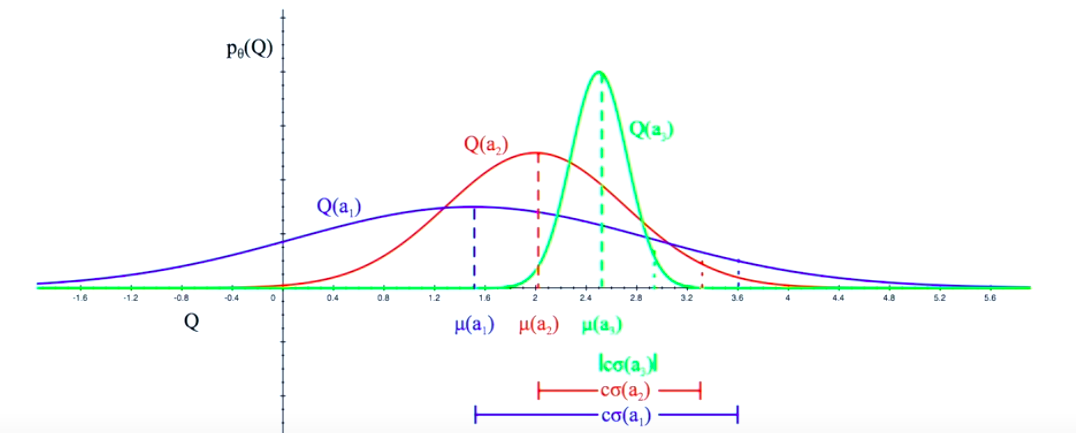
\includegraphics[width=\linewidth]{img/rl/ucb-bandits.png}
    \caption{Example of the Bayesian Beliefs over Reward}
    \label{fig:ucb-bayesian-bandits}
\end{figure}

If we have the case of Bernouli bandits, we can use the Beta distributions, which will be parametrized by the number of times we have gotten a zero and a one, i.e. $Q_t(a) = \beta(N_t(R = 0 | a), N_t(R = 1 | a))$.

Computing the posterior may be a lot harder for general examples. We have several ways to solve for the correct action given the posterior distributions.

\subsubsection{Upper Confidence Bound - Bayesian}

\begin{itemize}
    \item We compute the Posterior over the action values ($p(R_t | \theta, a)$)
    \item We pick an upper confidence bound, eg. standard deviation ($U_t(a) = \sigma$)
    \item We act in a way that maximizes $Q_t(a) + U_t(a)$
\end{itemize}

\subsubsection{Probability Matching}

We will select each action with the probability of it being optimal.
\begin{equation}
    \pi_t(a) = p(q(a) = max_{a^\prime} q(a^\prime) \vert H_{t-1})
\end{equation}
The probability may be difficult in general to get this probability analytically.

\subsubsection{Thomson Sampling}

We try to sample from the probability over the reward of each actions, and then select greedily.
\begin{equation}
    \pi_t(a) = \mathbb{E}[\mathcal{I}(Q_t(a) = max_{a^\prime} Q_t(a^\prime))] = p(q(a) = max_{a^\prime} q(a^\prime))
\end{equation}
This achives the Logrithmic lower bound of regret.

\subsubsection{Information State Space}

If we can quantify the value of information gained in terms of future rewards that we gain given the information. This is a Markov Decision Process over the internal observation states. (We will need to know $p(\tilde{s^\prime} \vert a, \tilde{s})$).
\begin{itemize}
    \item Solvable using Model Free Reinforcement Learning (Q-Learning)
    \item Solvable using Model Based Bayesian Reinforcement Learning (Gittens Indices)
\end{itemize}
This can be unwieldy and not scalable.


\subsection{Policy Based Methods}

Below is the definition of the policy, soft-max over action values, where the values H are just preferences and do not bear a direct correspondance to the action/state values.
\begin{equation}
    \pi(a) = \frac{e^{H_t(a)}}{\sum_b e^{H_t(b)}}
\end{equation}
Now we want to do gradient ascent over the value of the rewards, updating our preferences.
\begin{equation}
    \theta = \theta + \alpha \nabla_\theta \mathbb{E}[R_t | \theta]
\end{equation}


\begin{theorem}[Log Likelihood trick]{thm:log-likelihood-trick}
    We are computing the gradient for the Bandits, this is also known as the Reinforce trick (Williams, 1992).
    \begin{eqnarray}
        \nabla_\theta \mathbb{E}[R_t \vert \theta]
        &=& \nabla_\theta \sum_a \pi_\theta(a) \mathbb{E}[R_t \vert A_t = a] \\
        &=& \sum_a q(a) \nabla_\theta \pi_\theta(a) \\
        &=& \sum_a q(a) \frac{\pi_\theta(a)}{\pi_\theta(a)} \nabla_\theta \pi_\theta(a) \\
        &=& \sum_a \pi_\theta(a) q(a) \frac{\nabla_\theta \pi_\theta(a)}{\pi_\theta(a)} \\
        &=& \mathbb{E}[R_t \frac{\nabla_\theta \pi_\theta(A_t)}{\pi_\theta(A_t)}] \\
        &=& \mathbb{E}[R_t \nabla_\theta log \pi_\theta(A_t)] \\
    \end{eqnarray}
    We have converted a gradient over expectation into an expectation over a gradient, so now we can sample from the gradient of the distribution to be able to perform stochastic gradient descent.
\end{theorem}

Stochastic Gradient Ascent is now $\mathbf{\theta = \theta + \alpha R_t \nabla_0 log(\pi_0(A_t))}$

In the case of SoftMax over action preferences, we have:
\begin{eqnarray}
    H_{t+1}(a) &=& H_t(a) + \alpha R_t \frac{\partial log \pi_t(A_t)}{\partial H_t(a)} \\
    &=& H_t(a) + \alpha R_t (\mathcal{I}(a = A_t) - \pi_t(a)) \\
    \implies H_{t+1}(a) &=& H_t(a) + \alpha R_t \times \begin{cases}
        (1 - \pi_t(a)) \; \text{if}\; a = A_t \\
        (-\pi_t(a)) \; \text{if}\; a \neq A_t
    \end{cases}
\end{eqnarray}
So we are increasing the preferences of actions with higher rewards and pushing down the preferences of the actions even without taking them, therefore it's not the same as value.

We also note that the sum of probabilities over all actions is always 1, so we can add a baseline (constant independent of $\theta$ and $a$) to the reward without changing the preferences. But it does change the variance of the update. So
\textbf{performance can improve by adding a baseline like negative of the mean till now}.

\section{Dynamic Programming to solve MDPs}

The discount factor affects the goal we are going after.
